\documentclass{standalone}
\usepackage{tikz}
\usetikzlibrary{patterns, positioning}

\begin{document}
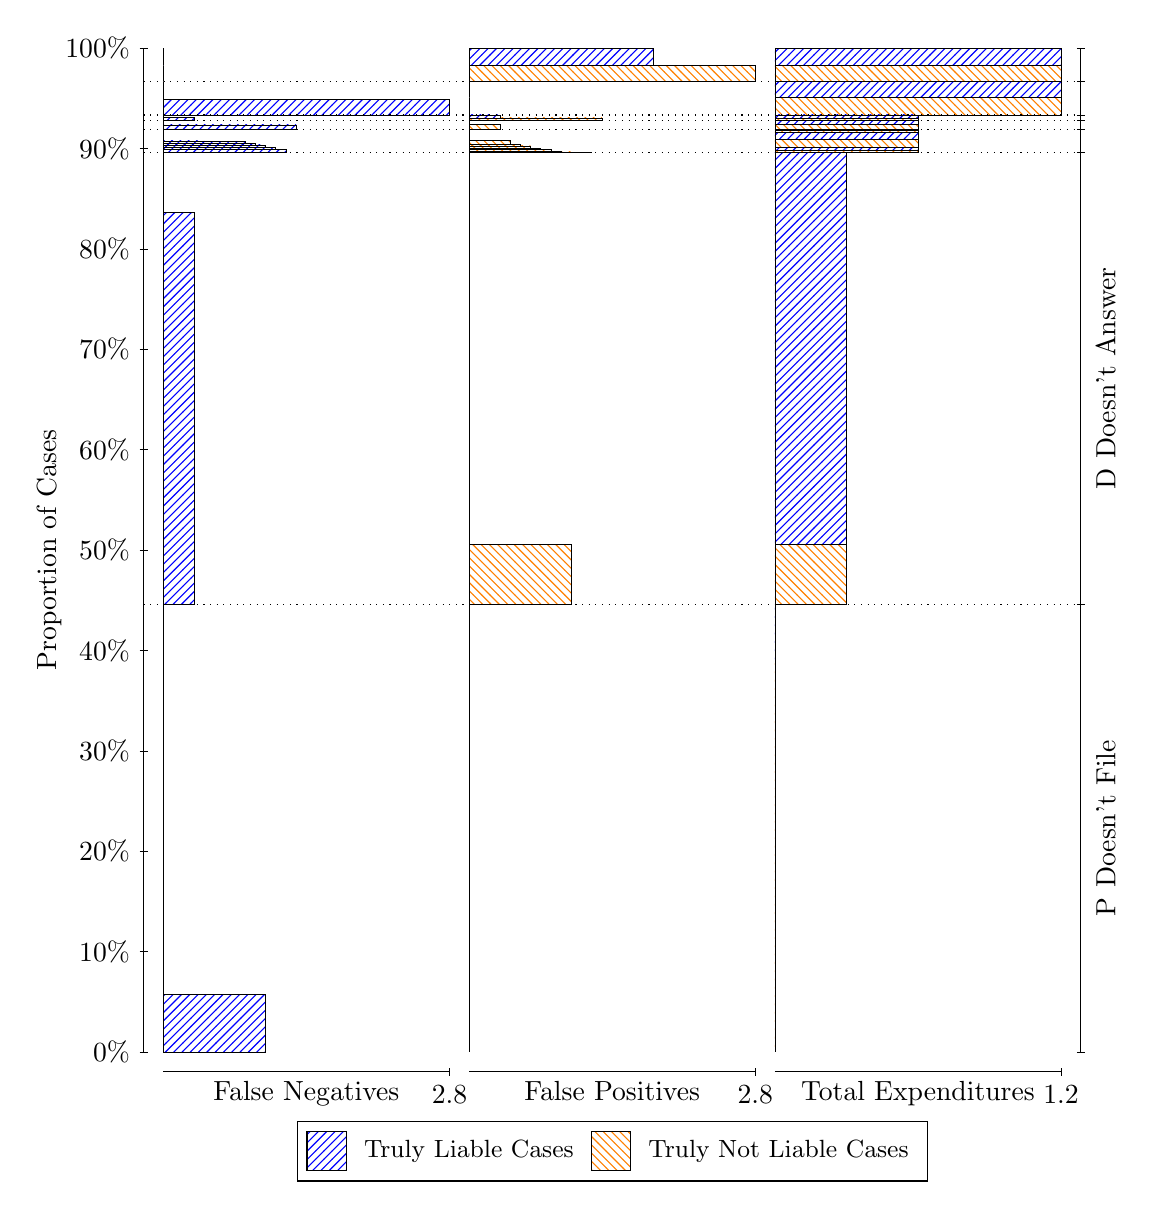
\begin{tikzpicture}
\draw[black, very thin] (1.5,1.75) -- (1.5,14.5);
\node[rotate=90, anchor=center] at (0.3, 8.125) {Proportion of Cases};
\draw[black, very thin] (1.45,1.75) -- (1.55,1.75);
\node[anchor=east] at (1.45, 1.75) {0\%};
\draw[black, very thin] (1.45,3.025) -- (1.55,3.025);
\node[anchor=east] at (1.45, 3.025) {10\%};
\draw[black, very thin] (1.45,4.3) -- (1.55,4.3);
\node[anchor=east] at (1.45, 4.3) {20\%};
\draw[black, very thin] (1.45,5.575) -- (1.55,5.575);
\node[anchor=east] at (1.45, 5.575) {30\%};
\draw[black, very thin] (1.45,6.85) -- (1.55,6.85);
\node[anchor=east] at (1.45, 6.85) {40\%};
\draw[black, very thin] (1.45,8.125) -- (1.55,8.125);
\node[anchor=east] at (1.45, 8.125) {50\%};
\draw[black, very thin] (1.45,9.4) -- (1.55,9.4);
\node[anchor=east] at (1.45, 9.4) {60\%};
\draw[black, very thin] (1.45,10.675) -- (1.55,10.675);
\node[anchor=east] at (1.45, 10.675) {70\%};
\draw[black, very thin] (1.45,11.95) -- (1.55,11.95);
\node[anchor=east] at (1.45, 11.95) {80\%};
\draw[black, very thin] (1.45,13.225) -- (1.55,13.225);
\node[anchor=east] at (1.45, 13.225) {90\%};
\draw[black, very thin] (1.45,14.5) -- (1.55,14.5);
\node[anchor=east] at (1.45, 14.5) {100\%};

\draw[black, very thin] (13.4,1.75) -- (13.4,14.5);
\draw[black, very thin] (13.35,1.75) -- (13.45,1.75);
\node[anchor=west] at (13.35, 1.75) {};
\draw[black, very thin] (13.35,7.436) -- (13.45,7.436);
\node[anchor=west] at (13.35, 7.436) {};
\draw[black, very thin] (13.35,13.173) -- (13.45,13.173);
\node[anchor=west] at (13.35, 13.173) {};
\draw[black, very thin] (13.35,13.471) -- (13.45,13.471);
\node[anchor=west] at (13.35, 13.471) {};
\draw[black, very thin] (13.35,13.579) -- (13.45,13.579);
\node[anchor=west] at (13.35, 13.579) {};
\draw[black, very thin] (13.35,13.65) -- (13.45,13.65);
\node[anchor=west] at (13.35, 13.65) {};
\draw[black, very thin] (13.35,14.074) -- (13.45,14.074);
\node[anchor=west] at (13.35, 14.074) {};
\draw[black, very thin] (13.35,14.5) -- (13.45,14.5);
\node[anchor=west] at (13.35, 14.5) {};

\draw[black, very thin, pattern color=blue, pattern=north east lines] (1.75,1.75) rectangle (3.0476,2.4834);
\draw[black, very thin, pattern color=orange, pattern=north west lines] (1.75,2.4834) rectangle (1.75,7.436);
\draw[black, very thin, pattern color=blue, pattern=north east lines] (1.75,7.436) rectangle (2.1393,12.416);
\draw[black, very thin, pattern color=orange, pattern=north west lines] (1.75,12.416) rectangle (1.75,13.173);
\draw[black, very thin, pattern color=blue, pattern=north east lines] (1.75,13.173) rectangle (3.3071,13.215);
\draw[black, very thin, pattern color=blue, pattern=north east lines] (1.75,13.215) rectangle (3.1774,13.235);
\draw[black, very thin, pattern color=blue, pattern=north east lines] (1.75,13.235) rectangle (3.0476,13.269);
\draw[black, very thin, pattern color=blue, pattern=north east lines] (1.75,13.269) rectangle (2.9179,13.271);
\draw[black, very thin, pattern color=blue, pattern=north east lines] (1.75,13.271) rectangle (2.9179,13.286);
\draw[black, very thin, pattern color=blue, pattern=north east lines] (1.75,13.286) rectangle (2.7881,13.31);
\draw[black, very thin, pattern color=blue, pattern=north east lines] (1.75,13.31) rectangle (2.6583,13.314);
\draw[black, very thin, pattern color=blue, pattern=north east lines] (1.75,13.314) rectangle (2.5286,13.318);
\draw[black, very thin, pattern color=blue, pattern=north east lines] (1.75,13.318) rectangle (2.3988,13.319);
\draw[black, very thin, pattern color=blue, pattern=north east lines] (1.75,13.319) rectangle (2.269,13.32);
\draw[black, very thin, pattern color=orange, pattern=north west lines] (1.75,13.32) rectangle (1.75,13.471);
\draw[black, very thin, pattern color=blue, pattern=north east lines] (1.75,13.471) rectangle (3.4369,13.523);
\draw[black, very thin, pattern color=orange, pattern=north west lines] (1.75,13.523) rectangle (1.75,13.579);
\draw[black, very thin, pattern color=blue, pattern=north east lines] (1.75,13.579) rectangle (2.1393,13.616);
\draw[black, very thin, pattern color=orange, pattern=north west lines] (1.75,13.616) rectangle (1.75,13.65);
\draw[black, very thin, pattern color=blue, pattern=north east lines] (1.75,13.65) rectangle (5.3833,13.851);
\draw[black, very thin, pattern color=orange, pattern=north west lines] (1.75,13.851) rectangle (1.75,14.074);
\draw[black, very thin, pattern color=orange, pattern=north west lines] (1.75,14.074) rectangle (1.75,14.275);
\draw[black, very thin, pattern color=blue, pattern=north east lines] (1.75,14.275) rectangle (1.75,14.5);
\draw[black, very thin, pattern color=orange, pattern=north west lines] (5.6333,1.75) rectangle (5.6333,6.7026);
\draw[black, very thin, pattern color=blue, pattern=north east lines] (5.6333,6.7026) rectangle (5.6333,7.436);
\draw[black, very thin, pattern color=orange, pattern=north west lines] (5.6333,7.436) rectangle (6.931,8.1934);
\draw[black, very thin, pattern color=blue, pattern=north east lines] (5.6333,8.1934) rectangle (5.6333,13.173);
\draw[black, very thin, pattern color=orange, pattern=north west lines] (5.6333,13.173) rectangle (7.1905,13.174);
\draw[black, very thin, pattern color=orange, pattern=north west lines] (5.6333,13.174) rectangle (7.0607,13.175);
\draw[black, very thin, pattern color=orange, pattern=north west lines] (5.6333,13.175) rectangle (6.931,13.18);
\draw[black, very thin, pattern color=orange, pattern=north west lines] (5.6333,13.18) rectangle (6.8012,13.183);
\draw[black, very thin, pattern color=orange, pattern=north west lines] (5.6333,13.183) rectangle (6.6714,13.208);
\draw[black, very thin, pattern color=orange, pattern=north west lines] (5.6333,13.208) rectangle (6.5417,13.224);
\draw[black, very thin, pattern color=orange, pattern=north west lines] (5.6333,13.224) rectangle (6.4119,13.258);
\draw[black, very thin, pattern color=orange, pattern=north west lines] (5.6333,13.258) rectangle (6.2821,13.278);
\draw[black, very thin, pattern color=orange, pattern=north west lines] (5.6333,13.278) rectangle (6.1524,13.324);
\draw[black, very thin, pattern color=blue, pattern=north east lines] (5.6333,13.324) rectangle (5.8929,13.325);
\draw[black, very thin, pattern color=blue, pattern=north east lines] (5.6333,13.325) rectangle (5.7631,13.325);
\draw[black, very thin, pattern color=blue, pattern=north east lines] (5.6333,13.325) rectangle (5.6333,13.471);
\draw[black, very thin, pattern color=orange, pattern=north west lines] (5.6333,13.471) rectangle (6.0226,13.527);
\draw[black, very thin, pattern color=blue, pattern=north east lines] (5.6333,13.527) rectangle (5.6333,13.579);
\draw[black, very thin, pattern color=orange, pattern=north west lines] (5.6333,13.579) rectangle (7.3202,13.614);
\draw[black, very thin, pattern color=blue, pattern=north east lines] (5.6333,13.614) rectangle (6.0226,13.65);
\draw[black, very thin, pattern color=orange, pattern=north west lines] (5.6333,13.65) rectangle (5.6333,13.873);
\draw[black, very thin, pattern color=blue, pattern=north east lines] (5.6333,13.873) rectangle (5.6333,14.074);
\draw[black, very thin, pattern color=orange, pattern=north west lines] (5.6333,14.074) rectangle (9.2667,14.275);
\draw[black, very thin, pattern color=blue, pattern=north east lines] (5.6333,14.275) rectangle (7.969,14.5);
\draw[black, very thin, pattern color=orange, pattern=north west lines] (9.5167,1.75) rectangle (9.5167,6.7026);
\draw[black, very thin, pattern color=blue, pattern=north east lines] (9.5167,6.7026) rectangle (9.5167,7.436);
\draw[black, very thin, pattern color=orange, pattern=north west lines] (9.5167,7.436) rectangle (10.425,8.1934);
\draw[black, very thin, pattern color=blue, pattern=north east lines] (9.5167,8.1934) rectangle (10.425,13.173);
\draw[black, very thin, pattern color=orange, pattern=north west lines] (9.5167,13.173) rectangle (11.333,13.203);
\draw[black, very thin, pattern color=blue, pattern=north east lines] (9.5167,13.203) rectangle (11.333,13.234);
\draw[black, very thin, pattern color=orange, pattern=north west lines] (9.5167,13.234) rectangle (11.333,13.335);
\draw[black, very thin, pattern color=blue, pattern=north east lines] (9.5167,13.335) rectangle (11.333,13.433);
\draw[black, very thin, pattern color=orange, pattern=north west lines] (9.5167,13.433) rectangle (11.333,13.452);
\draw[black, very thin, pattern color=blue, pattern=north east lines] (9.5167,13.452) rectangle (11.333,13.471);
\draw[black, very thin, pattern color=orange, pattern=north west lines] (9.5167,13.471) rectangle (11.333,13.527);
\draw[black, very thin, pattern color=blue, pattern=north east lines] (9.5167,13.527) rectangle (11.333,13.579);
\draw[black, very thin, pattern color=orange, pattern=north west lines] (9.5167,13.579) rectangle (11.333,13.614);
\draw[black, very thin, pattern color=blue, pattern=north east lines] (9.5167,13.614) rectangle (11.333,13.65);
\draw[black, very thin, pattern color=orange, pattern=north west lines] (9.5167,13.65) rectangle (13.15,13.873);
\draw[black, very thin, pattern color=blue, pattern=north east lines] (9.5167,13.873) rectangle (13.15,14.074);
\draw[black, very thin, pattern color=orange, pattern=north west lines] (9.5167,14.074) rectangle (13.15,14.275);
\draw[black, very thin, pattern color=blue, pattern=north east lines] (9.5167,14.275) rectangle (13.15,14.5);
\draw[black, dotted] (1.5,7.436) -- (13.4,7.436);
\draw[black, dotted] (1.5,13.173) -- (13.4,13.173);
\draw[black, dotted] (1.5,13.471) -- (13.4,13.471);
\draw[black, dotted] (1.5,13.579) -- (13.4,13.579);
\draw[black, dotted] (1.5,13.65) -- (13.4,13.65);
\draw[black, dotted] (1.5,14.074) -- (13.4,14.074);
\draw[black, very thin] (1.75,1.5) -- (5.3833,1.5);
\node[anchor=north] at (3.5667, 1.5) {False Negatives};
\draw[black, very thin] (5.3833,1.45) -- (5.3833,1.55);
\node[anchor=north] at (5.3833, 1.45) {2.8};

\draw[black, very thin] (5.6333,1.5) -- (9.2667,1.5);
\node[anchor=north] at (7.45, 1.5) {False Positives};
\draw[black, very thin] (9.2667,1.45) -- (9.2667,1.55);
\node[anchor=north] at (9.2667, 1.45) {2.8};

\draw[black, very thin] (9.5167,1.5) -- (13.15,1.5);
\node[anchor=north] at (11.333, 1.5) {Total Expenditures};
\draw[black, very thin] (13.15,1.45) -- (13.15,1.55);
\node[anchor=north] at (13.15, 1.45) {1.2};

\node[black, centered, rotate=90] at (13.72, 4.593) {P Doesn't File};
\node[black, centered, rotate=90] at (13.72, 10.305) {D Doesn't Answer};






\draw (7.449999999999999,1.5) node[draw=none] (baseCoordinate) {};
\begin{scope}[align=center]
        \matrix[scale=0.5, draw=black, below=0.5cm of baseCoordinate, nodes={draw}, column sep=0.1cm]{
            \node[rectangle, draw, minimum width=0.5cm, minimum height=0.5cm, pattern=north east lines, pattern color=blue] {}; &
            \node[draw=none, font=\small] (B) {Truly Liable Cases}; &
            \node[rectangle, draw, minimum width=0.5cm, minimum height=0.5cm, pattern=north west lines, pattern color=orange] {}; &
            \node[draw=none, font=\small] (B) {Truly Not Liable Cases}; \\
            };
\end{scope}

\end{tikzpicture}
\end{document}